\documentclass[]{article}
\usepackage{lmodern}
\usepackage{amssymb,amsmath}
\usepackage{ifxetex,ifluatex}
\usepackage{fixltx2e} % provides \textsubscript
\ifnum 0\ifxetex 1\fi\ifluatex 1\fi=0 % if pdftex
  \usepackage[T1]{fontenc}
  \usepackage[utf8]{inputenc}
\else % if luatex or xelatex
  \ifxetex
    \usepackage{mathspec}
  \else
    \usepackage{fontspec}
  \fi
  \defaultfontfeatures{Ligatures=TeX,Scale=MatchLowercase}
\fi
% use upquote if available, for straight quotes in verbatim environments
\IfFileExists{upquote.sty}{\usepackage{upquote}}{}
% use microtype if available
\IfFileExists{microtype.sty}{%
\usepackage{microtype}
\UseMicrotypeSet[protrusion]{basicmath} % disable protrusion for tt fonts
}{}
\usepackage[margin=1in]{geometry}
\usepackage{hyperref}
\hypersetup{unicode=true,
            pdftitle={Network structure from rich but noisy data},
            pdfauthor={Natalia Garcia Martin \& Maud Lemercier},
            pdfborder={0 0 0},
            breaklinks=true}
\urlstyle{same}  % don't use monospace font for urls
\usepackage{natbib}
\bibliographystyle{plainnat}
\usepackage{graphicx,grffile}
\makeatletter
\def\maxwidth{\ifdim\Gin@nat@width>\linewidth\linewidth\else\Gin@nat@width\fi}
\def\maxheight{\ifdim\Gin@nat@height>\textheight\textheight\else\Gin@nat@height\fi}
\makeatother
% Scale images if necessary, so that they will not overflow the page
% margins by default, and it is still possible to overwrite the defaults
% using explicit options in \includegraphics[width, height, ...]{}
\setkeys{Gin}{width=\maxwidth,height=\maxheight,keepaspectratio}
\IfFileExists{parskip.sty}{%
\usepackage{parskip}
}{% else
\setlength{\parindent}{0pt}
\setlength{\parskip}{6pt plus 2pt minus 1pt}
}
\setlength{\emergencystretch}{3em}  % prevent overfull lines
\providecommand{\tightlist}{%
  \setlength{\itemsep}{0pt}\setlength{\parskip}{0pt}}
\setcounter{secnumdepth}{5}
% Redefines (sub)paragraphs to behave more like sections
\ifx\paragraph\undefined\else
\let\oldparagraph\paragraph
\renewcommand{\paragraph}[1]{\oldparagraph{#1}\mbox{}}
\fi
\ifx\subparagraph\undefined\else
\let\oldsubparagraph\subparagraph
\renewcommand{\subparagraph}[1]{\oldsubparagraph{#1}\mbox{}}
\fi

%%% Use protect on footnotes to avoid problems with footnotes in titles
\let\rmarkdownfootnote\footnote%
\def\footnote{\protect\rmarkdownfootnote}

%%% Change title format to be more compact
\usepackage{titling}

% Create subtitle command for use in maketitle
\newcommand{\subtitle}[1]{
  \posttitle{
    \begin{center}\large#1\end{center}
    }
}

\setlength{\droptitle}{-2em}

  \title{Network structure from rich but noisy data}
    \pretitle{\vspace{\droptitle}\centering\huge}
  \posttitle{\par}
    \author{Natalia Garcia Martin \& Maud Lemercier}
    \preauthor{\centering\large\emph}
  \postauthor{\par}
      \predate{\centering\large\emph}
  \postdate{\par}
    \date{2018-10-17}

\usepackage{stmaryrd}
\usepackage{color}
\usepackage[ruled, vlined]{algorithm2e}

\usepackage{float}

\begin{document}
\maketitle
\begin{abstract}
We have implemented an R package to estimate the parameters of
exponential random graph models (ERG models), in the case where the data
consists of noisy observations of the underlying hidden structure. The
first part of this report focusses on the Bernouilli (or Erdos Renyi)
model, performing inference via the Expectation Maximization algorithm,
while the second part explores other ERG models, for which Bayesian
parameter estimation is more challenging.
\end{abstract}

\hypertarget{introduction}{%
\section{Introduction}\label{introduction}}

\hypertarget{problem-formulation-and-motivation}{%
\subsection{Problem formulation and
motivation}\label{problem-formulation-and-motivation}}

The true network structure is drawn from \(P(A|\theta_A)\). We will
later constrain this distribution to belong to the exponential random
graph models family. The observations of the network are supposed to be
noisy. The network structure and the observations are related to one
another by \(P(data|A,\theta_Y)\). Our aim is to infer the parameters
\(\theta=\{\theta_A,\theta_Y\}\) through the posterior distribution
\(P(\theta|data)\).
\[P(\theta|data)\propto \sum_AP(data|A,\theta_Y)P(A|\theta_A)P(\theta)\]
This optimisation problem is hard since the function is often non
convex, might have many local maxima and no analytical solutions. In our
model, as illustrated on Figure \ref{fig:graph_model}, we have two
unknowns: the latent variables and the parameters. We also suppose that
the underlying network is probed \(k\) times.

\begin{figure}[H]
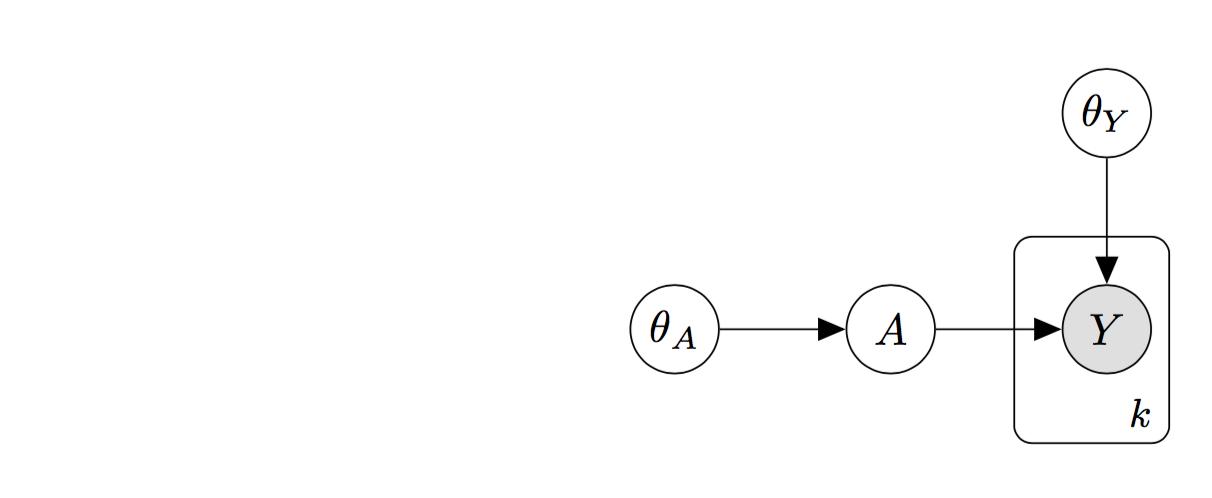
\includegraphics[width=0.65\linewidth]{GM2} \caption{\label{fig:graph_model}Graphical Model}\label{fig:pressure}
\end{figure}

In this report, we consider unweighted undirected networks,
characterised by an \(n \times n\) symmetric adjacency matrix \(A\),
having elements \(A_{i,j} = 1\) if nodes \(i\) and \(j\) are connected
by an edge and \(0\) otherwise. Similarly, we note \(Y_{i,j}^{(k)}\) the
edge measurement between node \(i\) and \(j\) at time \(k\).

\hypertarget{network-models}{%
\subsection{Network models}\label{network-models}}

\hypertarget{bernoulli-erdosrenyi-model}{%
\subsubsection{Bernoulli (Erdős--Rényi)
model}\label{bernoulli-erdosrenyi-model}}

The Bernoulli or Erdős--Rényi model is one of the simplest models for
random networks. Starting with \(n\) isolated vertices, for any pair of
nodes \((i, j)\) an edge is added with probability \(\rho>0\). This step
is repeated for the \(\binom{n}{2}=n(n-1)/2\) pairs of nodes. This
network is determined by the number of nodes \(n\), the probability of
edge formation \(\rho\) and the total number edges \(m\) and can be
expressed as either \(G(n,\rho)\) or \(G(n,m)\). We will use the former
notation. Since there are \(\binom{n}{2}\) pairs of nodes in the
network, the expected number of edges is given by \(\binom{n}{2}\rho\).
Similarly, the expected number of 2-stars is \(\binom{n}{3}\rho^2\) and
the expected number of triangles is \(\binom{n}{3}\rho^3\). The degree
\(deg(j)\) of a node \(j\) is defined as the number of edges connected
to it. Given the adjacency matrix \(A\), this is
\[ deg(j)=\sum_{i}{A_{i,j}}.\]

The average degree of the graph is then given by the average of the
individual nodes degrees. For a Bernoulli graph, the probability that a
given node has degree \(d\) is the product of \(a)\) the probability
that \(d\) links are present, \(b)\) the probability that the remaining
potential links are missing, and \(c)\) the number of combinations in
which we can select the \(d\) links out of the potential \(n-1\). Hence,
they follow a Binomial distribution:

\[ P(deg(j)=d)=p_d=\binom{n-1}{d}\rho^d(1-\rho)^{n-1-d} \]

with expected degree \(\rho(n-1)\). For large \(n\) and small \(\rho\),
this distribution can be approximated by a Poisson distribution with
parameter \(\rho(n-1)\). Due to all pairs of nodes having the same
probability of edge formation, the Erdős--Rényi model is not appropriate
to represent social networks, where edges tend to form between nodes
which already share common connections.\\

\hypertarget{ergm-model}{%
\subsubsection{ERGM model}\label{ergm-model}}

Exponential random graph models (ERGM) are a family of probability
distributions on graphs. Let \(\mathcal{A}_n\) be the set of all graphs
on \(n\) vertices, and consider the following model, where
\(\theta_i,~i=1,2,...,m\) are real valued parameters, and
\(T_i,~i=1,2,...,m\) are real valued statistics defined on
\(\mathcal{A}_n\). Possible sufficient statistics for such models are
the degree of the vertices, the number of edges, the number of k-stars,
the number of triangles, or the number of connected components. Altering
these features allows us to construct networks which resemble social
relationships. For example, triadic closure is a common occurrence in
friendship networks, where as explained before, nodes with common
neighbours are prone to form ties between them, resulting in a large
number of triangles. The general form for an ERGM is

\[
\begin{aligned}
P(\mbox{A}=a|\theta)&=\frac{1}{Z(\theta)}\exp\left(\sum_{i=1}^m{\theta_iT_i(a)}\right) \\ &=\frac{1}{Z(\theta)}\exp\left[\theta^tT(a)\right],
\end{aligned}
\]

where \(Z(\theta)\) is a normalisation constant satisfying
\(Z(\theta)=\sum_{a \in \mathcal{A}_n}\exp\left[\theta^tT(a)\right]\)
and \(\theta,T(a) \in \mathbb{R}^m\) represent the vector of parameters
and the vector of sufficient statistics respectively. The 1-dimensional
case with \(\theta = \frac{\rho}{1-\rho}\) gives us the expression for
the Bernoulli graph.\\

\begin{figure}[H]

{\centering 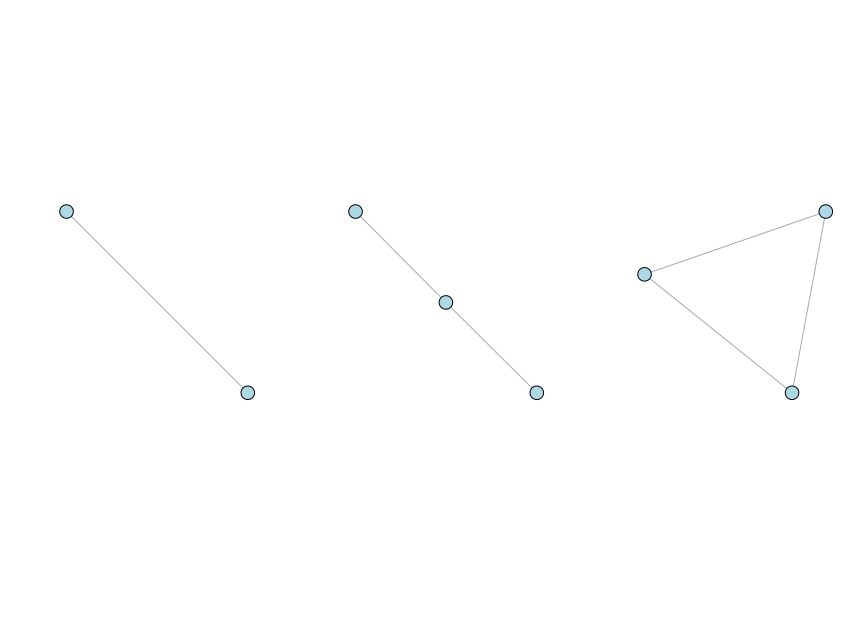
\includegraphics[width=0.6\linewidth,height=0.6\textheight]{triangle} 

}

\caption{\label{fig:triangle}Example of edge, 2-star, 3-star and triangle}\label{fig:unnamed-chunk-1}
\end{figure}

\hypertarget{methods}{%
\section{Methods}\label{methods}}

\hypertarget{inference-for-the-bernoulli-model}{%
\subsection{Inference for the Bernoulli
model}\label{inference-for-the-bernoulli-model}}

Since the underlying matrix \(A\) is symmetric, we consider the lower
triangular part of the matrix only and simulate the interactions for
each day \(k\) as edge observations \(Y_{i,j}^{(k)}\) for entries
\(i<j\). These observations are assumed to be independent Bernoulli
random variables conditioned on \(A_{i,j}\). Given that the prior
probability for a random edge is \(\rho\), the prior model for the
network is \[P(A|\rho)=\prod_{i<j}\rho^{A_{i,j}}(1-\rho)^{1-A_{i,j}}.\]

The data model is specified by \(P(\mbox{data}|A, \theta)\), where
\(data\) corresponds to the observed \(Y_{i,j}^{(k)}\). To simplify the
notations, we let \(E_{i,j}=\sum_kY_{i,j}^{(k)}\). Applying Bayes'
theorem,
\[P(A,\theta|\mbox{data})=\frac{P(\mbox{data}|A,\theta)P(A)P(\theta)}{P(\mbox{data})}.\]

Our aim is to find the parameters \(\theta\) that fix the relationship
between the network and the data in order to then estimate the actual
network structure. Summing over all the possible network structures
\(A\), we obtain the likelihood function
\[P(\theta|\mbox{data})=\sum_{A}{P(A,\theta|\mbox{data})}\]

which we want to maximise to find the best estimates of \(\theta\) given
the observed data. Taking logarithms in both sides and making use of the
Jensen inequality, we get \[\begin{aligned}
\log P(\theta|\mbox{data}) &= \log \sum_{A}{P(A,\theta|\mbox{data})} \\
                          &= \log \sum_{A} q(A)\frac{P(A,\theta|\mbox{data})}{q(A)} \\
                          &\geq \sum_{A} q(A) \log \frac{P(A,\theta|\mbox{data})}{q(A)},
\end{aligned}\]

where \(q(A)\) is any probability distribution over networks satisfying
\(\sum_{A}q(A)=1.\) The right hand size of the equation is maximised in
the case of equality, that is, when
\[q(A)=\frac{P(A,\theta|\mbox{data})}{ \sum_{A}P(A,\theta|\mbox{data})}.\]

Notice that \(q(A)=P(A|\mbox{data}, \theta)\). We will use this result
in order to estimate the parameters \(\theta\) and the true underlying
network \(A\) by employing an EM algorithm. We now define the
true-positive rate \(\alpha\) and the false-positive rate \(\beta\)
respectively as the probabilities of observing an edge when it actually
exists and observing it when it does not exist. We assume that the
priors for \(\alpha\), \(\beta\) and \(\rho\) are uniform in the
interval {[}0,1{]}. Then,

\[\begin{aligned}
P(\mbox{data}|A, \theta)
&=\prod_{i<j}\left(\alpha^{\sum_{k}Y_{i,j}^{(k)}}(1-\alpha)^{N_{i,j}-\sum_kY_{i,j}^{(k)}}\right)^{A_{i,j}}\left(\beta^{\sum_kY_{i,j}^{(k)}}(1-\beta)^{N_{i,j}-\sum_kY_{i,j}^{(k)}}\right)^{1-A_{i,j}} \\
&=\prod_{i<j}\left(\alpha^{E_{i,j}}(1-\alpha)^{N_{i,j}-E_{i,j}}\right)^{A_{i,j}}\left(\beta^{E_{i,j}}(1-\beta)^{N_{i,j}-E_{i,j}}\right)^{1-A_{i,j}}.
\end{aligned}\]

Combining this equation with the prior model for the network involving
\(\rho\) that we defined above, we obtain \[\begin{aligned}
P(A,\theta|\mbox{data})
&=\frac{1}{P(data)}\prod_{i<j}\left(\alpha^{E_{i,j}}(1-\alpha)^{N_{i,j}-E_{i,j}}\right)^{A_{i,j}}\left(\beta^{E_{i,j}}(1-\beta)^{N_{i,j}-E_{i,j}}\right)^{1-A_{i,j}} p(A)p(\theta) \\
&=\frac{1}{P(data)}\prod_{i<j}\left(\rho \alpha^{E_{i,j}}(1-\alpha)^{N_{i,j}-E_{i,j}}\right)^{A_{i,j}}\left((1-\rho)\beta^{E_{i,j}}(1-\beta)^{N_{i,j}-E_{i,j}}\right)^{1-A_{i,j}}.
\end{aligned}\]

\hypertarget{the-em-expectation-maximization-algorithm}{%
\subsection{The EM (expectation-maximization)
algorithm}\label{the-em-expectation-maximization-algorithm}}

\textbf{E-step}

The expectation step consists in updating the posterior probabilities
with the previous estimates of the parameters.

\[q^{(t)}(A)=\frac{p(A,\hat{\theta}^{(t)}|\mbox{data})}{\sum_A{p(A,\hat{\theta}^{(t)}|\mbox{data})}}\]
\textbf{M-step}

The maximisation step consists in solving the tractable optimisation
problem:
\[\sum_Aq^{(t)}(A)\nabla_\theta \log~{p(A,\hat{\theta}^{(t+1)}|\mbox{data})}=0\]
With the Bernoulli model, the maximisation step is tractable, since we
have:
\[\begin{split}P(A,\theta|\mbox{data})&=\frac{1}{P(\mbox{data})}\prod_{i<j}\left(\rho \alpha^{E_{i,j}}(1-\alpha)^{N_{i,j}-E_{i,j}}\right)^{A_{i,j}}\left((1-\rho)\beta^{E_{i,j}}(1-\beta)^{N_{i,j}-E_{i,j}}\right)^{1-A_{i,j}}\end{split}.\]

To simplify the notations, let
\(Q_{i,j}=P(A_{i,j}=1|data,\theta)=\sum_{A}{q(A)A_{i,j}}.\)

\textbackslash{}begin\{algorithm\}
\((\alpha,\beta, \rho) \leftarrow (\alpha^{(0)},\beta^{(0)}, \rho^{(0)})\)
\textbackslash{} \textbackslash{} \While(stopping criterion is not met)
\Do \Begin E step:\textbackslash{}
\(~~~Q_{i,j} \leftarrow \frac{\rho\alpha^{E_{i,j}}(1-\alpha)^{N-E_{i,j}}}{\rho\alpha^{E_{i,j}}(1-\alpha)^{N-E_{i,j}}+(1-\rho)\beta^{E_{i,j}}(1-\beta)^{N-E_{i,j}}}\)\textbackslash{}
M step: \textbackslash{} \Begin
\(~~~\alpha \leftarrow \frac{\sum_{i<j}E_{i,j}Q_{i,j}}{N\sum_{i<j}Q_{i,j}}\)
\textbackslash{}
\(~~~\beta \leftarrow \frac{\sum_{i<j}E_{i,j}(1-Q_{i,j})}{N\sum_{i<j}(1-Q_{i,j})}\)
\textbackslash{}
\(~~~\rho \leftarrow \frac{1}{{n \choose 2}}\sum_{i<j}Q_{i,j}\) \End
\End \Return{$Q,\alpha,\beta, \rho}\$ \textbackslash{}end\{algorithm\}

\hypertarget{inference-for-the-ergm-model}{%
\subsection{Inference for the ERGM
model}\label{inference-for-the-ergm-model}}

The aim of this section is to discuss how a bayesian estimation of the
parameters \(\theta=\{\theta_A, \theta_Y\}\) can be performed. In our
case, we cannot use a vanilla Metropolis Hastings algorithm with
\(p(\theta|Y)\) as a target distribution, for the following reasons:

\begin{itemize}
\item
  The normalising constant \(Z(\theta)\) is intractable. This problem is
  would also arise in the case where the network is completely observed.
\item
  The likelihood appearing in the acceptance ratio is intractable, since
  we would have to sum over all the states that the hidden variable
  \(A\) can take, with \(A\) a binary vector of size \(n\).
\end{itemize}

\[\alpha_{MH}(\theta,\theta')= 1 \land \frac{p(Y|\theta')p(\theta')q(\theta|\theta')}{p(Y|\theta)p(\theta)q(\theta'|\theta)}\]

\[p(Y|\theta)=\sum_Ap(Y|\theta,A)p(A|\theta) \]

\hypertarget{pseudolikelihood-estimation}{%
\subsection{Pseudolikelihood
estimation}\label{pseudolikelihood-estimation}}

\hypertarget{markov-chain-monte-carlo-maximum-likelihood-estimation-mcmc-mle}{%
\subsection{Markov Chain Monte Carlo Maximum Likelihood estimation
(MCMC-MLE)}\label{markov-chain-monte-carlo-maximum-likelihood-estimation-mcmc-mle}}

\hypertarget{the-exchange-algorithm}{%
\subsection{The Exchange Algorithm}\label{the-exchange-algorithm}}

The exchange algorithm (\cite{murray2012mcmc}) falls within the class of
\emph{auxiliary variable approaches}, which consist in introducing an
auxiliary variable \(u\) with a well-chosen conditional density
\(f(u|\theta,x)\) so that the intractable normalizing function cancels
out in the Metropolis-Hastings acceptance probability. In the case of
the exchange algorithm, this conditional density is
\(\frac{h(u|\theta)}{Z(\theta)}\).

The exchange algorithm augments the state from \(\theta\) to
\((\theta, \theta', u)\) and targets the augmented joint density

\[\begin{split}\pi(\theta,\theta',u|x) & \propto p(\theta)L(\theta|x)q(\theta'|\theta)L(\theta'|u) \\ & = p(\theta)\frac{h(x|\theta)}{Z(\theta)}q(\theta'|\theta)\frac{h(u|\theta')}{Z(\theta')}\end{split}\].
with a symmetric swapping proposal between the states
\(\{\theta',\theta\}\) and \(\{\theta,\theta'\}\). Therefore the
acceptance probability is

\[\alpha=min \left\{1,\frac{\pi(\theta',\theta,u|x)}{\pi(\theta,\theta',u|x)}\right\}=min\left\{1,\frac{p(\theta')h(x|\theta')h(u|\theta)q(\theta|\theta')}{p(\theta)h(x|\theta)h(u|\theta')q(\theta'|\theta)}\right\}\]

\begin{figure}[H]

{\centering 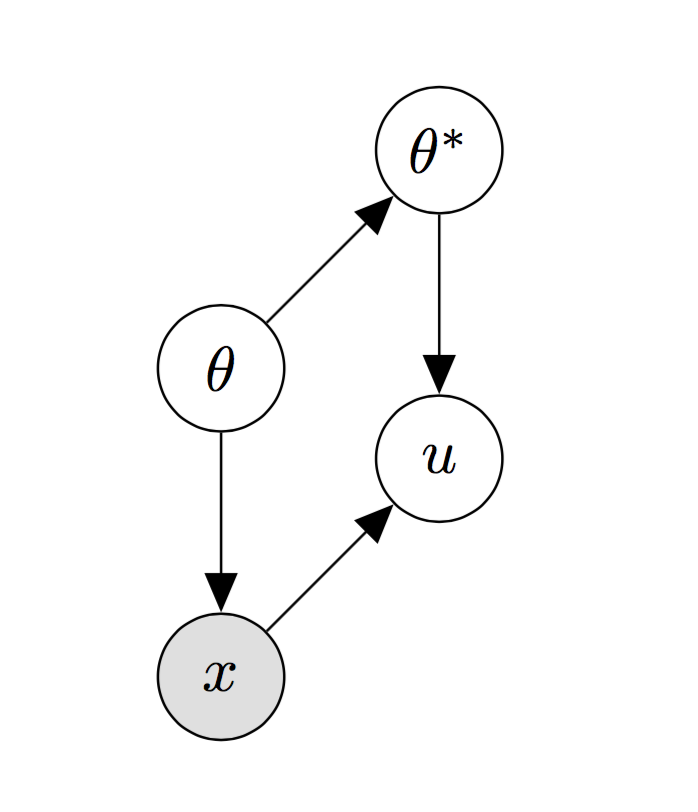
\includegraphics[width=0.2\linewidth,height=0.2\textheight]{exchange} 

}

\caption{\label{fig:triangle}The augmented model}\label{fig:unnamed-chunk-2}
\end{figure}

\begin{algorithm}[H]
 Given $\theta_n \in \Theta$ at the $n^{th}$ iteration \\
 1. Propose $\theta' \sim q(\cdot|\theta_n)$ \\ 
 2. Generate the auxiliary variable $u \sim \frac{h(\cdot|\theta')}{Z(\theta')}$ \\ 
 3. Accept $\theta_{n+1}$ with probability $\alpha = min\left\{1, \frac{p(\theta')h(x|\theta')h(u|\theta_n)q(\theta_n|\theta')}{p(\theta_n)h(x|\theta_n)h(u|\theta')q(\theta'|\theta_n)}\right\}$\\
 ~~~~Reject otherwise
 \caption{Exchange algorithm}
\end{algorithm}

\hypertarget{the-double-metropolis-hastings-algorithm}{%
\subsection{The Double Metropolis-Hastings
algorithm}\label{the-double-metropolis-hastings-algorithm}}

\begin{algorithm}[H]
 Given $\theta_n \in \Theta$ at the $n^{th}$ iteration \\
 1. Propose $\theta' \sim q(\cdot|\theta_n)$ \\ 
 2. Generate the auxiliary variable using $m$ MH-updates 
 ~~$u \sim T^m_{\theta'}(.|x)$ \\ 
3. Accept $\theta_{n+1}$ with probability $\alpha = min\left\{1, \frac{p(\theta'){\color{blue}T^m_{\theta'}(x|u)}h(u|\theta_n)q(\theta_n|\theta')}{p(\theta_n)h(x|\theta_n){\color{blue}T^m_{\theta'}(u|x)}q(\theta'|\theta_n)}\right\}$\\
 ~~~~Reject otherwise 
 \caption{Double Metropolis-Hastings algorithm}
\end{algorithm}

\hypertarget{results}{%
\section{Results}\label{results}}

\hypertarget{tests-on-simulated-data}{%
\subsection{Tests on simulated data}\label{tests-on-simulated-data}}

\textbf{Dataset}

In this section, we propose to validate the model's estimates using a
synthetic dataset for which the ground truth network and the noisy
observations are generated via a predefined probabilistic model. We
simulate a network with \(n=\) 100 vertices, and we set \(\rho=\) 0.1.
The noisy observations are then simulated for \(k=\) 5 days, with true
positive rate \(\alpha=\) 0.6 and false positive rate \(\beta=\) 0.009.
Our stopping criterion is met when the absolute value of the difference
of all parameter values after an iteration is less than \(\epsilon=\)
0.001.

\textbf{Results}

In this setting, the stopping criterion is met after 12 iterations. The
figure below, shows the comparison of the ground truth network with the
inferred network (obtained by thresholding the posterior probabilities
at \(t=\) 0.5), where the size of the nodes is proportional to their
degree.

\begin{figure}
\centering
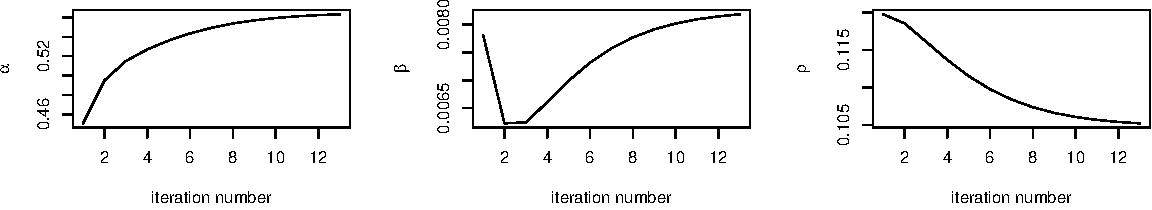
\includegraphics{report_files/figure-latex/unnamed-chunk-4-1.pdf}
\caption{\label{fig:comparison}(left) Ground truth underlying network
(right) Inferred underlying network}
\end{figure}

\begin{figure}[H]

{\centering 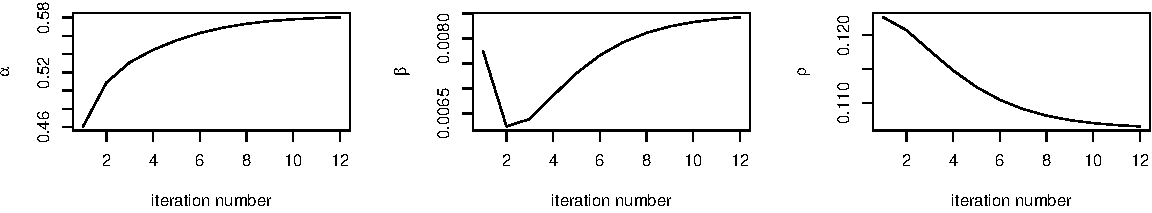
\includegraphics{report_files/figure-latex/unnamed-chunk-5-1} 

}

\caption{\label{fig:figs} Convergence of the parameter estimates}\label{fig:unnamed-chunk-5}
\end{figure}

\[
\centering\begin{tabular}{|c|c|}\hline Precision & 0.9957806 \\ \hline Recall & 0.9309665 \\ \hline Accuracy & 0.9925253 \\ \hline F-measure & 0.9622834 \\ \hline\end{tabular}\]

The figure below shows the influence of the number of repeated
observations \(k\) on the performances of the algorithm.

\begin{figure}[H]

{\centering 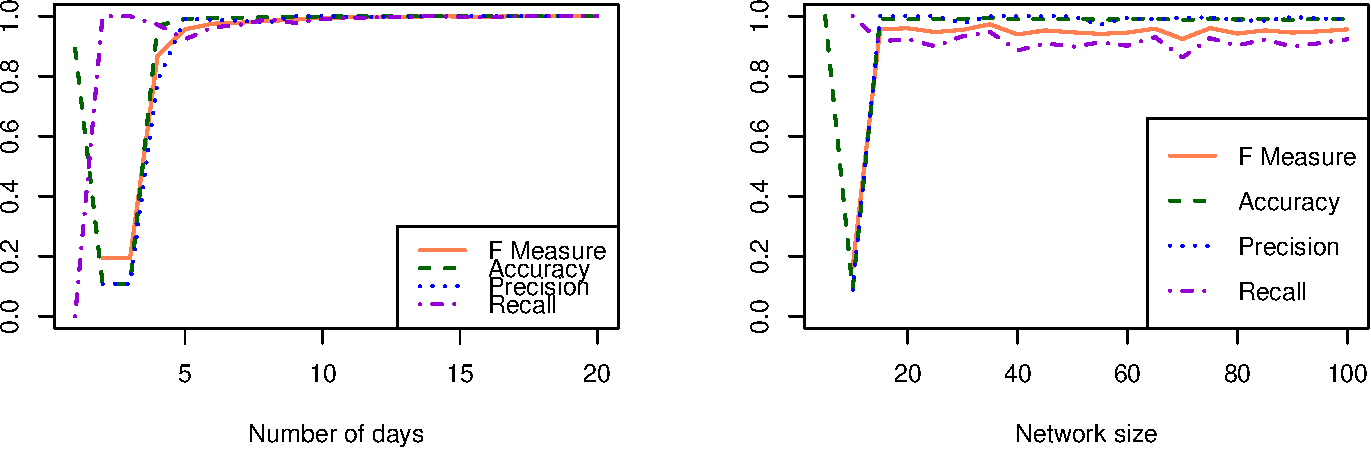
\includegraphics{report_files/figure-latex/unnamed-chunk-6-1} 

}

\caption{\label{fig:figs}Performance metrics versus the number of repeated observations k}\label{fig:unnamed-chunk-6}
\end{figure}

\hypertarget{discussion}{%
\section{Discussion}\label{discussion}}

\nocite{
morris2008specification,
eagle2006reality,
everitt2012bayesian,
korber2018bayesian,
jin2013bayesian,
newman2018network,
koskinen2010analysing,
everitt2017marginal,
murray2012mcmc,
hunter2006,
park2018bayesian,
strauss1990pseudolikelihood,
snijders2002markov,
schmid2017exponential}

\bibliography{references.bib}


\end{document}
